\chapter{Ablation study} \label{sec:ablation}
In this section, we investigate the sensitivity of our model to the described design choices and hyperparameter values.
Throughout the experiments, we keep the same base parameters as described in the experimental setup.
Similarly, the DBLP dataset is used throughout as it provides a wide range of features suitable for the evaluation of all supported tasks.

% ====================================================
\section{Auxiliary Embedding Ratio} \label{sec:abl:aux_emb}
To address the incompleteness constraints, $MGTCOM$ introduces auxiliary embeddings for nodes without features.
Zero-vector features are used for nodes that are unseen during training and don't have their own feature vector to encourage its inference from neighboring nodes.
While doing this introduces performance benefits, for large datasets it may not be possible to store the auxiliary embeddings in memory.

We define a procedure to work around this scaling issue by noting that embeddings only need to be constructed for a fraction of the most important nodes.
This is due to scaling laws applicable to most real-world networks.
Specifically, in this experiment, we sort all the nodes without features by their degree and use a fraction of the highest degree nodes for auxiliary embeddings. Other nodes are given a zero-vector upon inference.

\begin{figure}[ht]
\centering

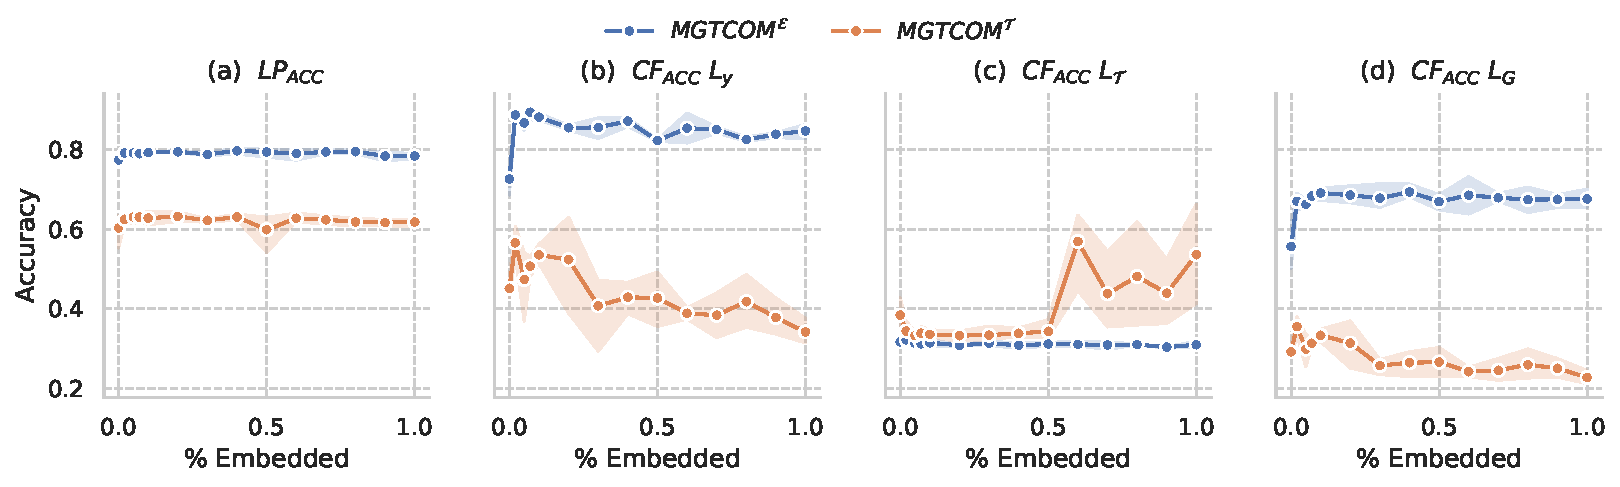
\includegraphics[width=\columnwidth]{resources/figs/embed_ratio.pdf}

\caption{
Performance results for topological $MGTCOM^{\mathcal{E}}$ and temporal $MGTCOM^{\mathcal{T}}$ models on various tasks where the ratio of auxiliary embedded nodes varies.
}
\label{fig:abl_embed_ratio}
\end{figure}
In \cref{fig:abl_embed_ratio} we see the results of the tasks specific models when the auxiliary ratio is varied.
From figure (a) we can observe that while auxiliary embeddings don't have a large influence during link prediction, they are in fact necessary on prediction tasks as figures (b), (c), and (d) indicate.
It can be rightfully deduced that embeddings are necessary for temporal tasks (figure (c)) since topology and content-based features are weakly correlated with temporal features.

% ====================================================
\section{Meta-topological features}
Meta-topological features are an important part of multimodal graphs.
In this experiment, we aim to determine the importance of meta-topology in our evaluation setting.
We evaluate the performance measures on heterogeneous and homogeneous variants of the DBLP dataset.
By varying convolutional layers between Heterogeneous Graph Transformer and GraphSAGE \cite{csirosdata61StargazersStellargraphStellargraph2018} (each edge type has a separate set of weights), we additionally aim to determine the importance of meta-topology-based attention used during the aggregation step.

\begin{figure}[ht]
\centering

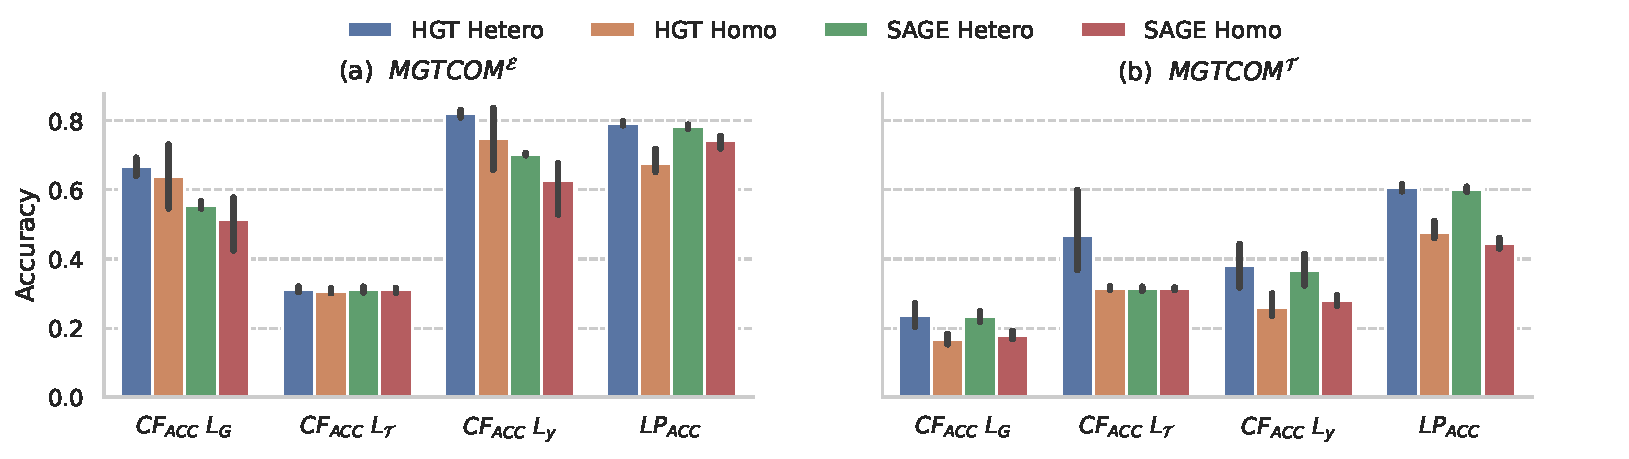
\includegraphics[width=\columnwidth]{resources/figs/abl_meta.pdf}

\caption{
Performance results for (a) topological $MGTCOM^{\mathcal{E}}$ and (b) temporal $MGTCOM^{\mathcal{T}}$ models, on prediction tasks for heterogeneous and homogeneous variants of the DBLP dataset.
To determine the importance of meta-topological attention we vary the convolutional layers HGT and GraphSAGE (which is adopted for heterogeneous graphs).
}
\label{fig:ablation_meta}
\end{figure}

Overall in \cref{fig:ablation_meta} we see that the addition of meta-topological features has a positive effect on the classification performance of both topological as well as temporal models. 
This effect is especially pronounced on link prediction and topology-based classification tasks for the temporal model. 
The cause for this may be that while topological features are not provided during training, meta-topology still conveys enough information about the topology.

From the results, we see that meta-topology-based attention yields benefits in classification performance in contrast to naive aggregation techniques (improvement by ~10\%).

% ====================================================
\section{Trade-off Parameter} \label{sec:abl:aux_emb}
During analysis the trade-off parameters ($\beta^{\mathcal{E}}$, $\beta^{\mathcal{T}}$, $\beta^{\mathcal{C}}$) are used to guide the trained embeddings to favor specific tasks.
In this experiment, we explore the trade-off between temporal and topological tasks by varying value of $\beta^{\mathcal{E}}$, $\beta^{\mathcal{T}}$ while setting the constraint $1 = \beta^{\mathcal{E}}$ + $\beta^{\mathcal{T}}$. 
The clustering weight parameter $\beta^{\mathcal{C}}$ remains constant throughout as described in \cref{sec:exp_setup}.

In \cref{fig:abl_beta} (a) we can see an almost linear correlation between link prediction accuracy and the topological weight parameter $\beta^{\mathcal{E}}$.
On the other hand, in figures (b) and (d) we see a more logarithmic curve for topology correlated classification measures.
The most interesting takeaway is that while variance is quite high on the temporal classification task, its curve peaks at a value of 0.5.
In further work, it may be worth exploring this phenomenon in more detail. 
The most probable assumption would be that the temporal model still benefits from the fact that temporal features are weakly correlated with the topology.

\begin{figure}[ht!]
\centering

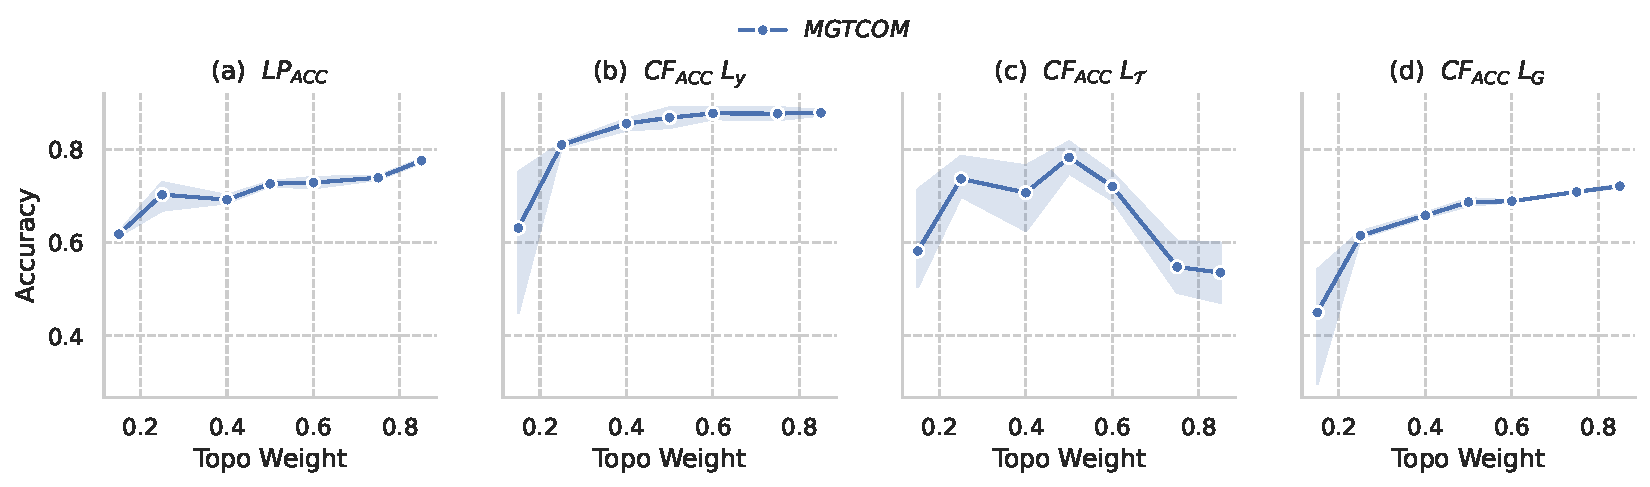
\includegraphics[width=\columnwidth]{resources/figs/abl_beta_topo.pdf}

\caption{
Performance of $MGTCOM$ model while varying topological loss weight parameter $\beta^{\mathcal{T}}$ under $1 = \beta^{\mathcal{E}}$ + $\beta^{\mathcal{T}}$ contraint.
}
\label{fig:abl_beta}
\end{figure}

% ====================================================
\section{Initial $K$ sensitivity}
In this section evaluate the sensitivity of the clustering results to the initial $K$ value selection.
While our method does not require setting the cluster to count $K$, it can still be set to find more accurate initial clustering, and help DPMM avoid local minima.
Specifically, we have varied the initial cluster count (init $K$) used for k-means initialization while keeping all other parameters fixed.

\begin{figure}[ht]
\centering

\subfigure[]{
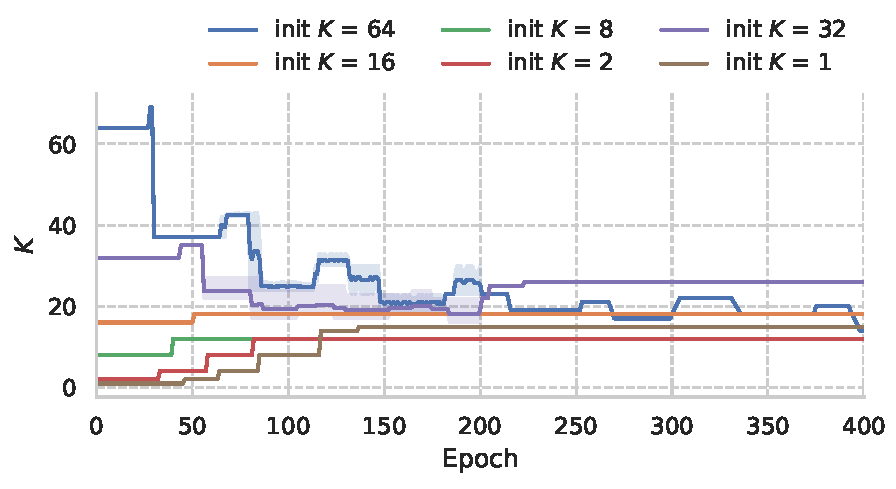
\includegraphics[width=0.48\textwidth]{resources/figs/abl_initk_k.pdf}
}
\subfigure[]{
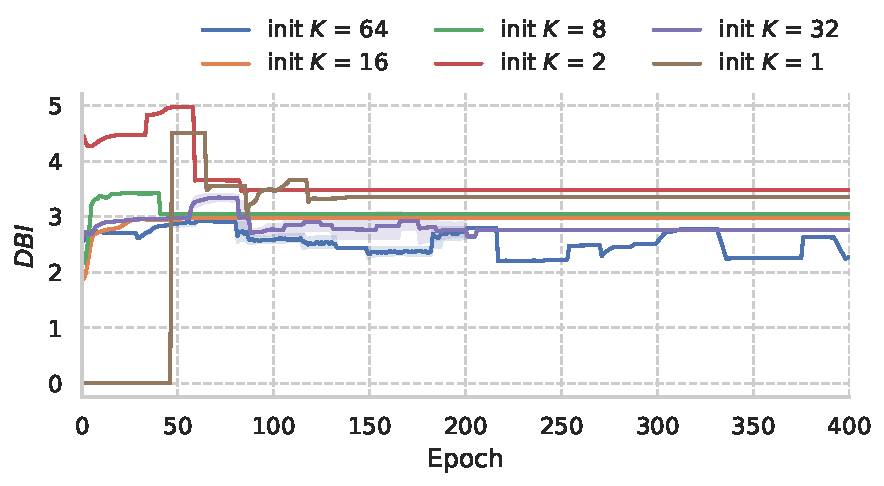
\includegraphics[width=0.48\textwidth]{resources/figs/abl_initk_dbi.pdf}
}

\caption{
(a) and (b): Cluster count progression during DPMM clustering given an initial cluster count (init $K$). The clustering is done on pre-trained $MGTCOM$ embeddings for the DBLP dataset.
}
\label{fig:ablation_k}
\end{figure}

In \cref{fig:ablation_k} (a) we see that despite varying starting values, all the runs converge at 12-18 cluster range.
Having a value that strongly deviates from the "optimal" cluster count causes a slower convergence since more split/merge operations are required.
We can see a similar pattern in the measured Davies-Bouldin index in \cref{fig:ablation_meta} (b).

% ====================================================
\section{Hyperparameter sensitivity} \label{sec:abl:hyperparam}
\begin{figure}[ht!]
\centering
\subfigure[]{
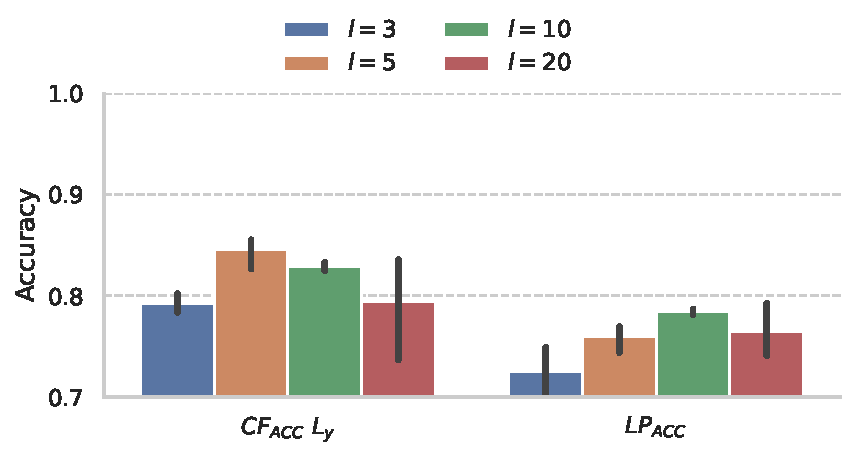
\includegraphics[width=0.47\textwidth]{resources/figs/tune_topo_rw_ctx.pdf}
}\quad
\subfigure[]{
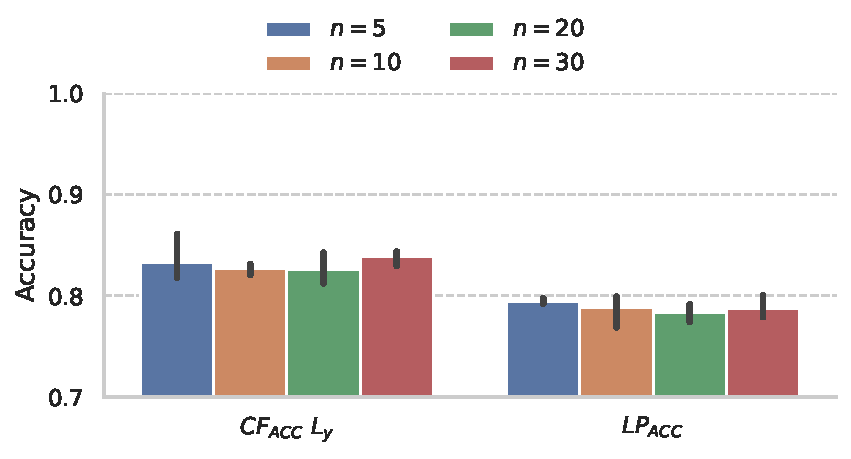
\includegraphics[width=0.47\textwidth]{resources/figs/tune_topo_rw_nwalks.pdf}
}\quad
\subfigure[]{
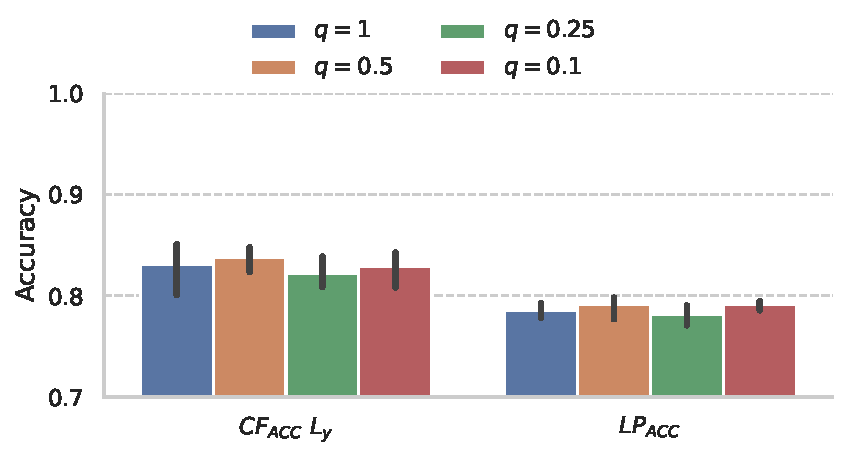
\includegraphics[width=0.47\textwidth]{resources/figs/tune_topo_rw_q.pdf}
}\quad
\caption{
Performance of $MGTCOM^{\mathcal{E}}$ model with varying (a) random walks length $l$, (b) number of random walks per node $n$, and (c) the exploration trade-off parameter $q$.
}
\label{fig:hyp_rw_topo}
\end{figure}    

In this part, the sensitivity of other hyperparameters on the model performance is discussed.
%
The node2vec random walk algorithm used for the topological task relies on parameters such as walk length $l$, the number of random walks $n$ for each node, and the exploration trade-off parameter $q$.
In \cref{fig:hyp_rw_topo} we see that while the choice of random walk length has a significant impact on link-prediction and classification performance (a), the model is not as sensitive to the other parameters.
A surprising observation is that the trade-off parameter does not significantly affect the productivity accuracy of ground communities ($CF_{ACC}$ $L_y$).
A possible explanation for this may be the fact that we use both random walk and neighborhood sampling algorithms making the trade-off ineffective.

\begin{figure}[ht!]
\centering
\subfigure[]{
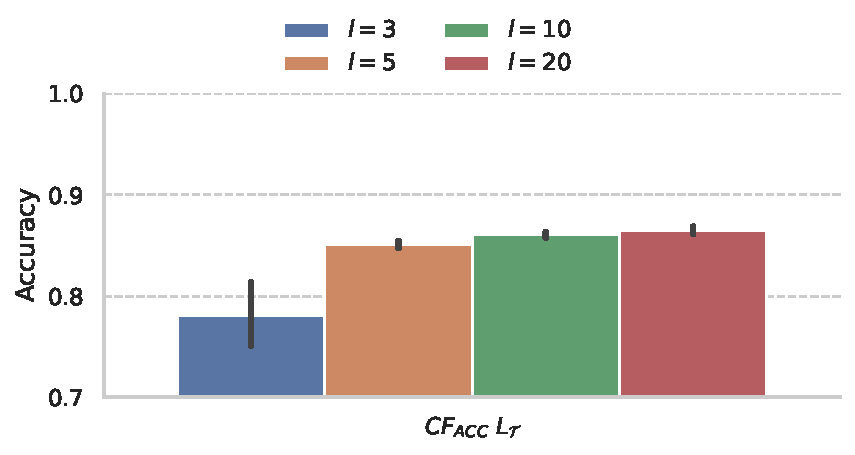
\includegraphics[width=0.47\textwidth]{resources/figs/tune_tempo_rw_ctx.pdf}
}\quad
\subfigure[]{
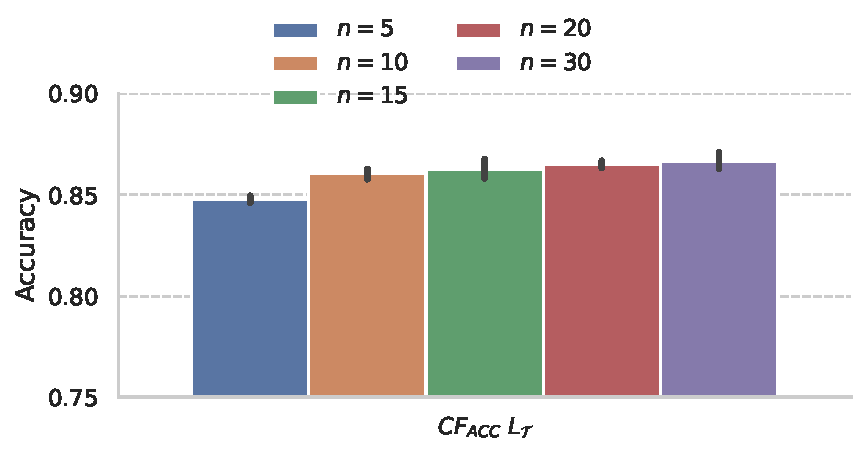
\includegraphics[width=0.47\textwidth]{resources/figs/tune_tempo_rw_nwalks.pdf}
}\quad
\caption{
Performance of $MGTCOM^{\mathcal{T}}$ model with varying (a) random walks length $l$ and (b) number of random walks per node $n$.
}
\label{fig:hyp_rw_tempo}
\end{figure}    

The ballroom walk algorithm introduced in \cref{sec:tempo_sampling} similarly relies on the hyperparameters walk length $l$ and the number of random walks started for each node $n$, though they serve a different purpose.
Increasing either the $l$ or the $n$ parameter only marginally increases the models performance at timestamp prediction (See \cref{fig:hyp_rw_tempo}).
For both parameters, there is a positive correlation between performance and an increase in the receptive field. 

\begin{figure}[ht!]
\centering
\subfigure[]{
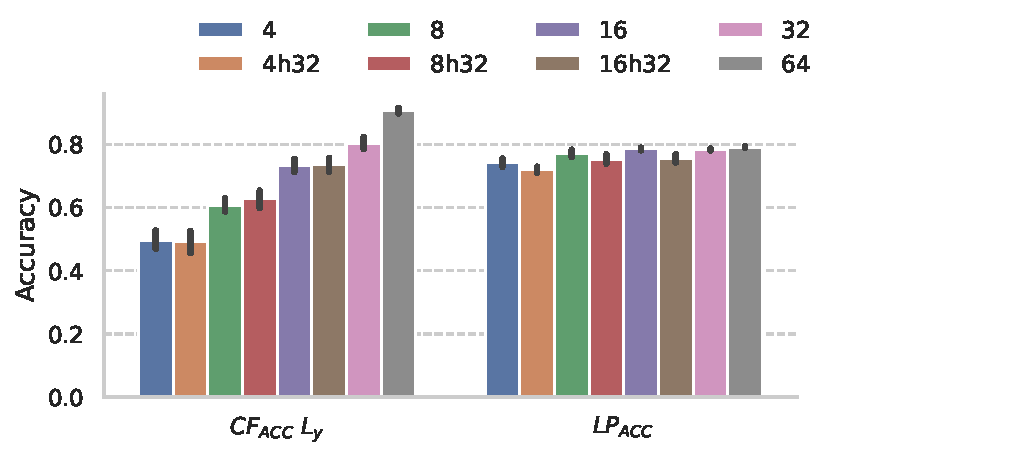
\includegraphics[width=0.47\textwidth]{resources/figs/tune_topo_reprdim.pdf}
}\quad
\subfigure[]{
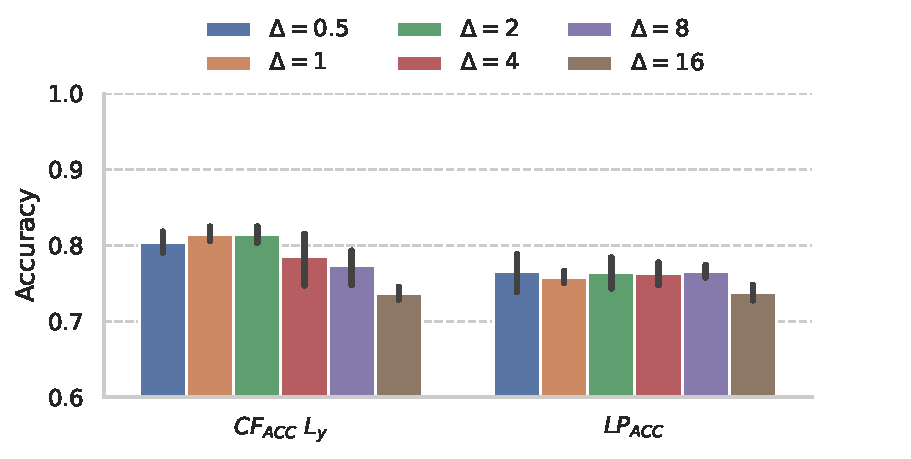
\includegraphics[width=0.47\textwidth]{resources/figs/tune_topo_margin.pdf}
}\quad
\subfigure[]{
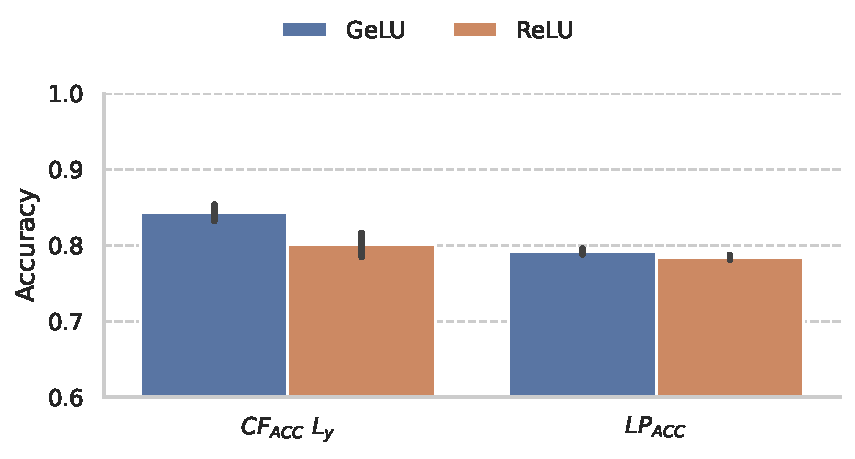
\includegraphics[width=0.46\textwidth]{resources/figs/tune_topo_activation.pdf}
}\quad
\caption{
Performance of $MGTCOM^{\mathcal{E}}$ model with varying (a) representation dimension $d$, (b) the margin ($\Delta$) parameter for the hinge loss, and (c) activation function.
}
\label{fig:hyp_rw_repr}
\end{figure}    

The most sensitive/important parameter for our model is the representation dimension size $d$.
In \cref{fig:hyp_rw_repr} (a) we plot the predictive performance of the topological model while varying the model representation dimension $d$ and the hidden representation dimension $h$ used in in-between layers of graph convolution.
The classification performance seems to benefit the most from a larger $d$, while link-prediction only sees a marginal improvement.
Moreover having hidden dimension size deviate from the representation dimension only seems to degrade the model performance.

In \cref{fig:hyp_rw_repr} (b) we vary the margin parameter of hinge loss. 
It is conventional to use $\Delta = 1$ if the similarity is bounded (as is in our case), therefore we can see the model performance degrade as the margin exceeds this threshold.
Increasing loss beyond $1$ amplifies the relative relevance of small loss samples, which in turn makes the model more prone to noise.

While constructing the network we found that the choice of activation function noticeably affects the model performance. 
Choosing GeLU over ReLU activation speeds up model convergence and gains a noticeable edge in classification tasks (See \cref{fig:hyp_rw_repr} (c)).

\begin{figure}[]
\centering

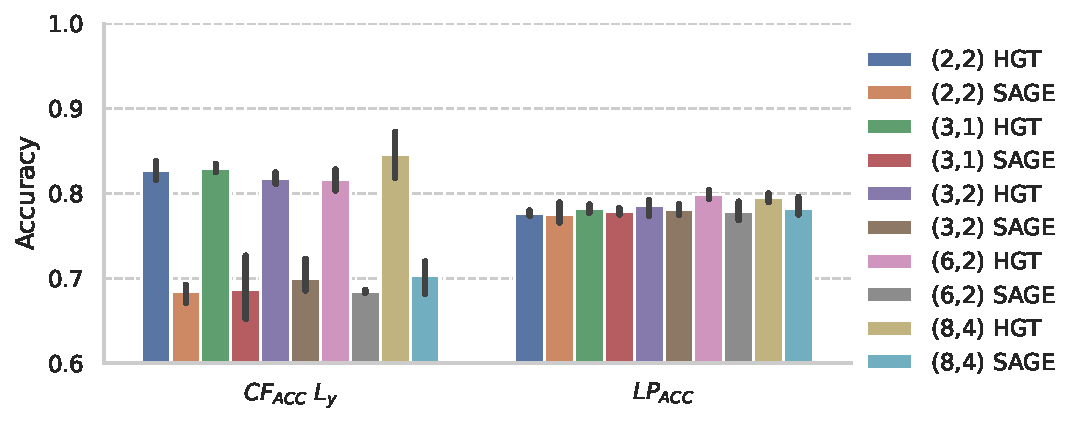
\includegraphics[width=0.6\columnwidth]{resources/figs/tune_topo_neigh.pdf}

\caption{
Performance of $MGTCOM^{\mathcal{E}}$ model with varying convolution layers. 
We vary the architecture by switching between Heterogeneous Graph Transformer (HGT) and Heterogenous GraphSAGE convolutional layers.
Similarly, we also modify the neighborhood size of each node within the two-layer convolution setup. 
Format $(x, y)$ represents the number of neighbors per node in the first ($x$) and second ($y$) layer respectively.
}
\label{fig:hyp_neigh}
\end{figure}

In \cref{fig:hyp_neigh} we vary the convolution architecture of the topological model and measure the resulting test performance.
As observed earlier HGT convolutional layers perform better since they introduce meta-topology-based attention. 
Varying the layer neighborhood size does not seem to affect the performance substantially, except for the fact that computed performance measures during training are a lot smoother throughout.

\begin{figure}[]
\centering
\subfigure[]{
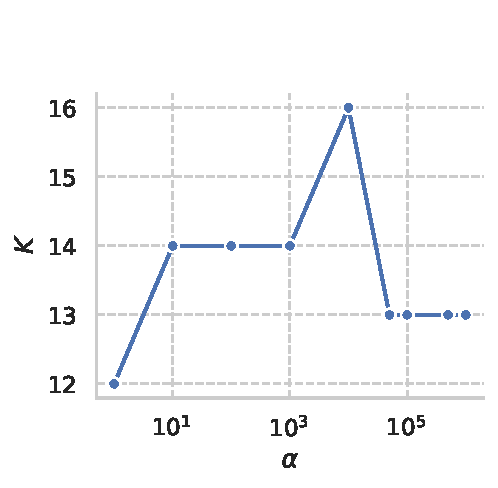
\includegraphics[width=0.3\textwidth]{resources/figs/cluster_alpha.pdf}
}\quad
\subfigure[]{
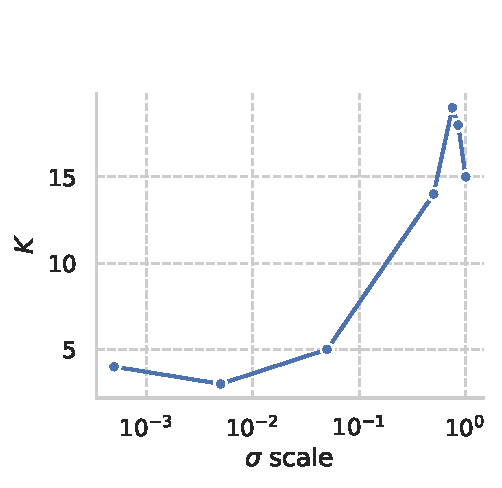
\includegraphics[width=0.3\textwidth]{resources/figs/cluster_sigma_scale.pdf}
}\quad \\
\subfigure[]{
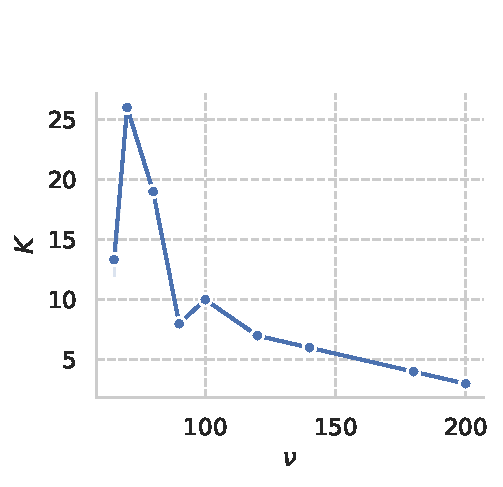
\includegraphics[width=0.3\textwidth]{resources/figs/cluster_nu.pdf}
}\quad
\subfigure[]{
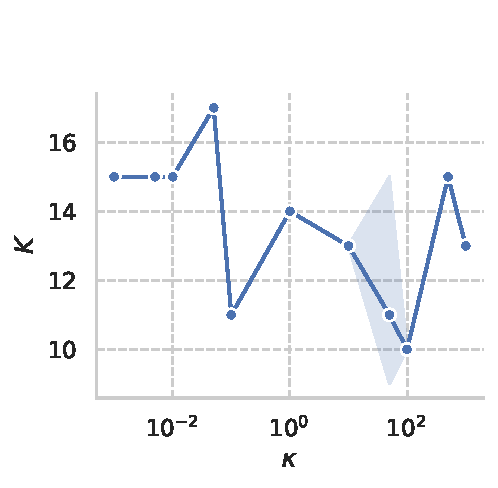
\includegraphics[width=0.3\textwidth]{resources/figs/cluster_kappa.pdf}
}\quad
\caption{
    Sensitivity of the resulting cluster count $K$ on the DPMM prior parameters (a) $\alpha$ the cluster concentration parameter, (b) the $\sigma$ scale parameter influencing the covariance of prior, (c) $\nu$ the degrees of freedom parameter for the Wishart prior distribution, and (d) $\kappa$ the concentration parameter of the Wishart prior distribution.
}
\label{fig:hyp_cluster}
\end{figure}

Finally, in \cref{fig:hyp_cluster} we analyze the sensitivity of the resulting cluster count to the chosen prior parameters for the DPMM algorithm.
We notice that the $\sigma$ scale and $\nu$ parameters have a linear correlation with the resulting number of clusters.
The $\sigma$ scale parameter influences the data-bound $W$ hyperparameter and is to be expected to have a great impact.
A larger prior covariance corresponds to a larger probability that any of the clusters are drawn from it and therefore results in a larger number of clusters.
On the contrary, a larger degree of freedom requires a larger amount of samples per cluster, therefore reducing the probability of smaller clusters.
We see a more noisy pattern from $\alpha$ and $\kappa$ concentration hyperparameters as they are not data-bound and are less effective when their value is much smaller than the total number of data points $N$.


